\documentclass[12pt]{article}

\usepackage[utf8]{inputenc}
\usepackage{datetime}
\usepackage{amsthm}
\usepackage{amsmath}
\usepackage{amssymb}
\usepackage{enumitem}
\usepackage[USenglish]{babel}
\usepackage{matlab-prettifier}
\usepackage{graphicx}
\usepackage[makeroom]{cancel}
\usepackage{afterpage}
\usepackage{capt-of}

\DeclareMathOperator*{\argmin}{arg\,min}
\DeclareMathOperator*{\argmax}{arg\,max}

\newcommand\independent{\protect\mathpalette{\protect\independenT}{\perp}}
\def\independenT#1#2{\mathrel{\rlap{$#1#2$}\mkern2mu{#1#2}}}

\newtheoremstyle{colon}{\topsep}{\topsep}{}{}{\bfseries}{:}{ }{}
\theoremstyle{colon}
\newtheorem{exercise}{Exercise}
\newtheorem*{answer}{Answer}

\title{ORFE 523: Convex and Conic Optimization \\ Homework 4}
\author{Zachary Hervieux-Moore}

\newdate{date}{11}{04}{2017}
\date{\displaydate{date}}

\begin{document}

\maketitle

\clearpage

\begin{exercise}
  A popular matrix norm in machine learning these days is the so-called \textit{nuclear norm}. The nuclear norm of a matrix $A \in \mathbb{R}^{m \times n}$ is given by
  \begin{gather*}
    \lVert A \rVert_* := \sum_{i=1}^{\min \{m,n\}} \sigma_i(A)
  \end{gather*}
  where $\sigma_i$ is the $i$-th singular value of $A$. There is considerable interest in this norm partly because it serves as the convex envelope of the function rank($A$) over the set $\{ A \in \mathbb{R}^{m \times n} : \lVert A \rVert_2 \leq 1 \}$.
  \begin{enumerate}[label=\arabic*)]
    \item Show that the dual norm of the spectral norm is the nuclear norm.
    \item Plot the unit ball of the nuclear norm for symmetric $2 \times 2$ matrices.
    \item Show that the problem of minimizing the nuclear norm of a matrix subject to arbitrary affine constraints can be cast as a semidefinite program.
  \end{enumerate}
\end{exercise}

\begin{answer}
  \leavevmode
  \begin{enumerate}[label=\arabic*)]
    \item We have that the spectral norm is
      \begin{gather*}
        \lVert A \rVert_2 = \max \{\lVert A x \rVert_2 : \lVert x \rVert_2 \leq 1 \}
      \end{gather*}
      Then its dual is
      \begin{gather*}
        \lVert A \rVert_{2*} = \max \{ \langle A, X \rangle : \lVert X \rVert_2 \leq 1 \}
      \end{gather*}
      We show that $\lVert A \rVert_{2*} = \lVert A \rVert_*$ by showing they are less than or equal to each other. Let $U \Sigma V^T$ be the SVD of $A$. Then, let $X = U V^T$. Their inner product is
      \begin{gather*}
        \langle A, X \rangle = \text{trace}(V \Sigma U^T U V^T) \\
        = \text{trace}(V \Sigma I V^T) = \text{trace}(\Sigma V^T V) \\
        = \text{trace}(\Sigma) = \lVert A \rVert_*
      \end{gather*}
      We also have that $\lVert X \rVert_2 = 1$ since $U V^T$ is orthogonal. Thus, we have showed $\lVert A \rVert_* \leq \max_{X : \lVert X \rVert_2 \leq 1} \langle A, X \rangle$

      Now suppose that $\lVert X \rVert_2 \leq 1$. Then
      \begin{gather*}
        \langle A, X \rangle = \text{trace}(V \Sigma U^T X) = \text{trace}(U^T X V \Sigma)
      \end{gather*}
      We note that spectral norm for the matrices $U^T$ and $V$ are less than 1 since they are orthonormal and $X$ by assumption.
      \begin{gather*}
        \lVert U^T X V \rVert_2 \leq \lVert U^T \rVert_2 \lVert X \rVert_2 \lVert V \rVert_2 \leq 1
      \end{gather*}
      Now let $X' = U^T X V$, which makes the trace of $\langle A, X' \rangle$ equal to
      \begin{gather*}
        = \text{trace}(X' \Sigma) = \sum_{i=1}^n \sigma_i x'_{ii} \leq \sum_{i=1}^n \sigma_i \lvert x'_{ii} \rvert
      \end{gather*}
      But we just showed that $\lVert X' \rVert_2 \leq 1$. Hence, we have
      \begin{gather*}
        = \text{trace}(X' \Sigma) \leq \sum_{i=1}^n \sigma_i = \lVert A \rVert_*
      \end{gather*}
      So, $\max_{X : \lVert X \rVert_2 \leq 1} \langle A, X \rangle \leq \lVert A \rVert_*$ and we conclude that
      \begin{gather*}
        \lVert A \rVert_{2*} = \max_{X : \lVert X \rVert_2 \leq 1} \langle A, X \rangle = \lVert A \rVert_*
      \end{gather*}

    \item Now let $S_2 = \{ M : M \in \mathbb{S}^{2 \times 2}, \lVert M \rVert_* \leq 1 \}$. Since $M$ is symmetric, we have that the singular values are precisely the absolute values of the eigenvalues. Thus, $\lVert M \rVert_* \leq 1 \implies \lvert \lambda_1 \rvert + \lvert \lambda_2 \rvert \leq 1$. This gives us four inequalities, $\pm \lambda_1 + \pm \lambda_2 \leq 1$. We also have that
      \begin{gather*}
        \text{det} \left( \begin{bmatrix} x & y/\sqrt{2} \\ y/\sqrt{2} & z \end{bmatrix} - \lambda I \right) = \lambda^2 - (x+z) \lambda + xz - y^2/2
      \end{gather*}
      Which means that the roots are
      \begin{gather*}
        \lambda = \frac{x+z \pm \sqrt{(x-z)^2 + 2y^2}}{2}
      \end{gather*}
      Combining these roots with the four inequalities before, we get the following inequalities
      \begin{gather*}
        -1 \leq x + z \leq 1 \\
        (x - z)^2 + 2 y^2 \leq 1
      \end{gather*}
      Consider the new variables $x' = \frac{1}{\sqrt{2}} x + \frac{1}{\sqrt{2}}z$, $y' = -\frac{1}{\sqrt{2}} x + \frac{1}{\sqrt{2}}z$, $z' = y$. Then we can write the above as
      \begin{gather*}
        -1 \leq \sqrt{2} x' \leq 1 \\
        y'^2 + z'^2 \leq 1/2
      \end{gather*}
      Thus, this is a cylinder with axis (1,0,1) passing through the origin whose top and bottom line on the plane $x+z = \pm 1$ and radius $1/\sqrt{2}$. The plot is below.

      \begin{center}
        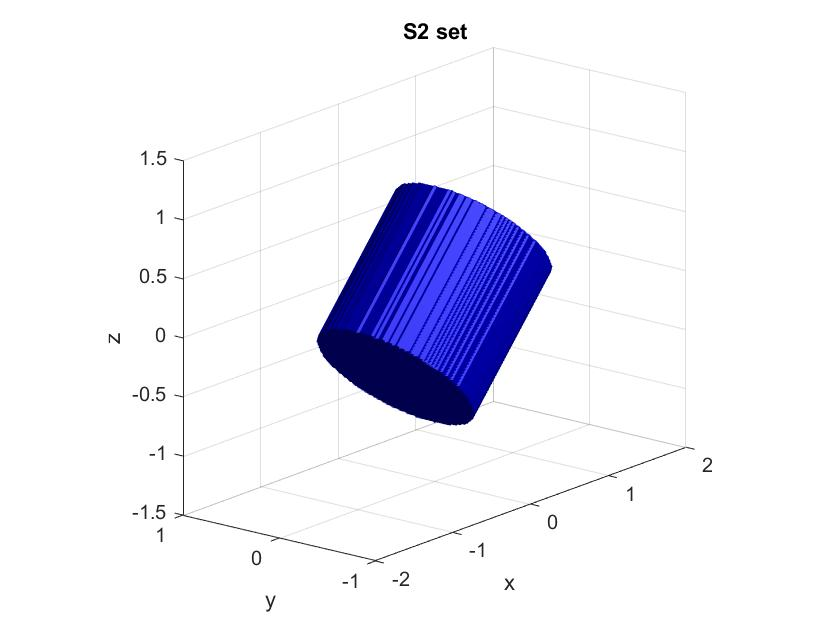
\includegraphics[width=0.8\textwidth]{cylinder.jpg}
        \captionof{figure}{Plot of $S_2$}
      \end{center}

    \item We wish first turn the nuclear norm into a definition similar to the SDP setting. To do this, we need the constraint $\lVert X \rVert_2 \leq 1$ to be some type of psd constraint. We define the matrix
      \begin{gather*}
        Y = \begin{bmatrix}
          I_n & X \\
          X^T & I_m
        \end{bmatrix}
      \end{gather*}
      Since $I_n \succ 0$, then, by Schur complement
      \begin{gather*}
        Y \succeq 0 \Longleftrightarrow I_m - X^T X \succeq 0 \Longleftarrow I_m \succeq X^T X
      \end{gather*}
      But, since $\lVert X \rVert_2 \leq 1$, then we have $x^T X^T X x \leq x^T x$ which is equivalent to $X^T X \preceq I_m$. Thus, $\lVert X \rVert_2 \leq 1 \Longleftrightarrow X^T X \preceq I_m \Longleftrightarrow 0 \preceq Y$. So now we rewrite the nuclear norm as
      \begin{gather*}
        \lVert A \rVert_* = \max_{Y \succeq 0} \langle A, X \rangle
      \end{gather*}
      We can get $Y$ into the objective by the following
      \begin{gather*}
        \lVert A \rVert_* = \frac{1}{2} \max_{Y \succeq 0} \left\langle \begin{bmatrix} 0 & A \\ A^T & 0 \end{bmatrix}, Y \right\rangle \\
        \implies \lVert A \rVert_* = \frac{1}{2} \max_{Y \succeq 0} \text{Trace} \left( \begin{bmatrix} 0 & A \\ A^T & 0 \end{bmatrix} Y \right)
      \end{gather*}
      Thus, we have turned the definition of the nuclear norm into an objective involving trace and psd constraints which is precisely what we want. But we make this a minimization problem by doing the typical double negation
      \begin{gather*}
        \lVert A \rVert_* = -\frac{1}{2} \min_{Y \succeq 0} -\text{Trace} \left( \begin{bmatrix} 0 & A \\ A^T & 0 \end{bmatrix} Y \right)
      \end{gather*}

      Now, we return to minimizing the nuclear norm and add in the arbitrary affine constraints
      \begin{gather*}
        \min_{\text{Trace}(C_i A) = b_i} \lVert A \rVert_* = \min_{\text{Trace}(C_i A) = b_i} -\frac{1}{2} \min_{Y \succeq 0} \text{Trace} \left( \begin{bmatrix} 0 & A \\ A^T & 0 \end{bmatrix} Y \right) \\
        = -\frac{1}{2} \min_{\substack{Y \succeq 0 \\ \text{Trace}(C_i A) = b_i}} -\text{Trace} \left( \begin{bmatrix} 0 & A \\ A^T & 0 \end{bmatrix} Y \right)
      \end{gather*}
      Which is an SDP.
  \end{enumerate}
\end{answer}

\clearpage

\begin{exercise}
  You are given a list of distances $d_{ij}$ for $\{i,j\} \in \{1, \mathellipsis, m\} \times \{1, \mathellipsis, m\}$. You would like to know whether there are points $x_i \in \mathbb{R}^n$, for some value of $n$, such that
  \begin{gather*}
    \lVert x_i - x_j \rVert_2 = d_{ij}, \quad \forall i,j
  \end{gather*}
  \begin{enumerate}[label=\arabic*)]
    \item Show that this problem can be formulated as a semidefinite program (SDP). If this SDP answers ``yes'', how would you recover $n$ and points $x_i$?
    \item Give an example of a set of distances that respect the triangle inequality but for which there does not exist an embedding in any dimension.
  \end{enumerate}
\end{exercise}

\begin{answer}
  \leavevmode
  \begin{enumerate}[label=\arabic*)]
    \item We can write the distances as $d_{ij} = X_{ii} + X_{jj} - 2X_{ij}$ where $X_{ij}$ is defined to be
      \begin{gather*}
        X_{ij} = \langle x_i, x_j \rangle
      \end{gather*}
      By symmetry of the inner product, $X$ is symmetric. This comes from the fact that
      \begin{gather*}
        d_{ij} = \lVert x_i - x_j \rVert_2^2 = \langle x_i, x_i \rangle + \langle x_j, x_j \rangle - 2 \langle x_i, x_j \rangle
      \end{gather*}
      Also, we have that $X$ is psd since for all $y \in \mathbb{R}^m$ we have
      \begin{gather*}
        y^T X y = \sum_{i,j = 1}^m \langle x_i, x_j \rangle y_i y_j = \lVert \sum_{i=1}^m y_i x_i \rVert_2^2 \geq 0
      \end{gather*}
      Conversely, to extract the distance matrix if such an $X$ existed ($X$ psd and $X_{ii} + X_{jj} - 2X_{ij} = d_{ij}$), we consider a Cholesky decomposition of $X = L L^T$ where $L \in \mathbb{R}^{m \times m}$. Then, $X_{ij} = l_i^T l_j$ and $d_{ij} = \lVert l_i - l_j \rVert_2^2$. Thus, we have shown that a distance matrix $d_{ij}$ exists if and only if there exists $X \in \mathbb{R}^{m \times m}$, $X$ psd, and $X_{ii} + X_{jj} - 2X_{ij} = d_{ij}$. This equates to testing feasibility of the SDP
      \begin{gather*}
        X \succeq 0 \\
        \text{Trace}((E_{ii} + E_{jj} - E_{ij}) X) = d_{ij}
      \end{gather*}
      Where $E_{ij}$ is the matrix with all zeroes except at entries $(i,j)$ and $(j,i)$ it is 1. Thus, we have $n = m$ and we recover the points $x_i$ by computing the Cholesky decomposition of $X$ and taking $x_i = l_i$.

    \item Consider the distance matrix
      \begin{gather*}
        d = \begin{bmatrix}
          0 & 1 & 1 & 1 \\
          1 & 0 & 1 & 1 \\
          1 & 1 & 0 & 2 \\
          1 & 1 & 2 & 0
        \end{bmatrix}
      \end{gather*}
      This satisfies the triangle inequality because $d_{ij} + d{jk} \geq 2$ for any $i \neq j \neq k$ and 2 is the largest distance in the matrix. From the previous part, we know that if an embedding exists, it exists in 4 dimensions. Now, wlog, we can place $x_1$ at the origin. Then $x_2, x_3, x_4$ all lie on the unit sphere as they are a unit away from the origin. Furthermore, we have that $\lVert x_3 - x_4 \rvert_2 = 2$ which implies they are diametrically opposed to each other. But then, the only way that $\lVert x_3 - x_2 \rvert_2 = 1$ and $\lVert x_4 - x_2 \rvert_2 = 1$ is if $x_2$ is also at the origin. But then $\lVert x_1 - x_2 \rVert_2 = 0 \neq 1$.
  \end{enumerate}
\end{answer}

\clearpage

\begin{exercise}
  Recall that the spectral radius of a matrix $A \in \mathbb{R}^{n \times n}$, denoted by $\rho(A)$, is the maximum of the absolute values of its eigenvalues. We call a matrix ``stable'' if $\rho(A) < 1$. Let us call a pair of real $n \times n$ matrices $\{ A_1, A_2 \}$ stable if $\rho(\Sigma) < 1$, for finite product $\Sigma$ out of $A_1$ and $A_2$. (For examples, $\Sigma$ could be $A_2 A_1, A_1 A_2, A_1 A_1,A_2A_1$, and so on).
  \begin{enumerate}[label=\arabic*)]
    \item Does the stability of $A_1$ and $A_2$ imply stability of the pair $\{A_1, A_2\}$?
    \item Prove (possibly using optimization) that the pair $\{A_1, A_2\}$ with
      \begin{gather*}
        A_1 = \frac{1}{4} \begin{bmatrix}
          -1 & -1 \\
          -4 & 0
        \end{bmatrix}, A_2 = \frac{1}{4} \begin{bmatrix}
          3 & 3 \\
          -2 & 1
        \end{bmatrix}
      \end{gather*}
      is stable.
  \end{enumerate}
\end{exercise}

\begin{answer}
  \begin{enumerate}[label=\arabic*)]
    \item No, this is not true. Consider
      \begin{gather*}
        A_1 = \begin{bmatrix}
          0.9 & 0.9 \\
          0 & 0.9
        \end{bmatrix} \text{ and } A_2 = \begin{bmatrix}
          0.9 & 0 \\
          0.9 & 0.9
        \end{bmatrix}
      \end{gather*}
      Then both the eigenvalues are 0.9 for both matrices. However, their product
      \begin{gather*}
        A_1 A_2 = \begin{bmatrix}
          1.62 & 0.81 \\
          0.81 & 0.81
        \end{bmatrix}
      \end{gather*}
      Has an eigenvalue of $\approx 2.12$ and so it is not stable.

    \item First, let us consider a finite product $\Sigma$. Suppose, for induction, that $\Sigma$ is stable and now we wish to multiply by another matrix $A_i$. Assume there exists $P \succ 0$ and $A_i^T P A_i \prec P$. One might recall the similarity to the Lyapunov theorem. Also, note that if $P \succeq 0$ then $\Sigma P \Sigma \succeq 0$. Since $x^T \Sigma^T P \Sigma x = (\Sigma x)^T P (\Sigma x) \geq 0$. Then we have
      \begin{gather*}
        A_i^T \Sigma^T P \Sigma A_i \preceq A_i^T P A_i \prec P
      \end{gather*}
      Where we used the last fact in step 1 and our assumption in step 2. Thus, by the Lyapunov theorem for quadratic functions, $\Sigma$ is stable. Now, let us create an SDP that finds a $P$ that satisfies our assumptions. This is shown below. The SDP, if it is feasible, will find $A_i^T P A_i \prec P$, $0 \prec P$. Since Matlab finds a solution, this pair is stable.

      \clearpage

      \textbf{Code Appendix:}

      \begin{lstlisting}[style=Matlab-editor, basicstyle=\scriptsize]
        clear;
        clc;

        A_1 = [-1,-1;-4,0]/4
        A_2 = [3,3;-2,1]/4
        epsilon = 0.1;

        cvx_begin sdp
            variable P(2,2)

            minimize(P(1,1));

            subject to

            A_1'*P*A_1 <= P + epsilon*eye(2,2)
            A_2'*P*A_2 <= P + epsilon*eye(2,2)
            P >= epsilon*eye(2,2)
        cvx_end
      \end{lstlisting}
  \end{enumerate}
\end{answer}

\clearpage

\begin{exercise}
  Consider a dynamical system $x_{k+1} = A x_k$, where $A \in \mathbb{R}^{n \times n}$. Suppose that the spectral radius of $A$ is strictly less than 1 and consider the set
  \begin{gather*}
    \mathcal{S} := \{ x \in \mathbb{R}^n : x^T x \leq 1 \}
  \end{gather*}
  Give an SDP-based algorithm that constructs a set $\mathcal{S}$' such that (i) $\partial S \cap \partial S'$ is nonempty, and (ii) if $x_0 \in \mathcal{S}'$, then $x_k \in \mathcal{S}$ for all $k$.
\end{exercise}

\begin{answer}
  First note that $\mathcal{S}$ is a sphere centered at the origin $\mathbb{R}^n$. Furthermore, since the dynamical system is linear and $\rho(A) < 1$. In essence, we need to find an ellipsoid that is contained in $\mathcal{S}$ yet touches the boundary. Furthermore, we need to make sure it stays in $\mathcal{S}$, thus, we need to find the $P$ of the quadratic Lyapunov function to make sure it remains in $\mathcal{S}$ because we will have $x^T A^T P A x < x^T P x$ which the right hand side is monotonically decreasing as it is our Lyapunov function. Since $\rho(A) < 1$ this system is GAS and so such a $P$ exists. Let us find it using an SDP.
  \begin{align*}
    \max_{\gamma, P \in \mathbb{S}^{n \times n}} \quad &\gamma \\
    \text{s.t. } \quad & A^T P A \preceq P \\
    & 0 \preceq P \\
    & \gamma I \preceq P
  \end{align*}
  Where the last constraint is used to ensure that the boundaries touch by maximizing the minimum eigenvalue. That is $\lambda_{\min}(P) = \gamma$. Now, let us define $\mathcal{S}'$ as
  \begin{gather*}
    \mathcal{S}' = \{ y \in \mathbb{R}^n : y^T P y \leq  \gamma \}
  \end{gather*}
  From our constraints we have $\gamma y^T I y \leq y^T P y$ which implies that $\gamma y^T y \leq y^T P y \leq \gamma$. This implies that $y^T y \leq 1$. Therefore $\mathcal{S}' \subseteq \mathcal{S}$. Furthermore, $\partial \mathcal{S}' \cap \partial \mathcal{S} \neq \emptyset$ since we can pick the eigenvector $\frac{v_{\min}}{\lVert v_{\min} \rVert}$ which has unit length and $\frac{v_{\min}^T}{\lVert v_{\min} \rVert} P \frac{v_{\min}}{\lVert v_{\min} \rVert} = \gamma \frac{v_{\min}^T}{\lVert v_{\min} \rVert} \frac{v_{\min}}{\lVert v_{\min} \rVert} = \gamma$. Thus, $\frac{v_{\min}}{\lVert v_{\min} \rVert} \in \mathcal{S}' \cap \partial \mathcal{S}$.
\end{answer}

\end{document}